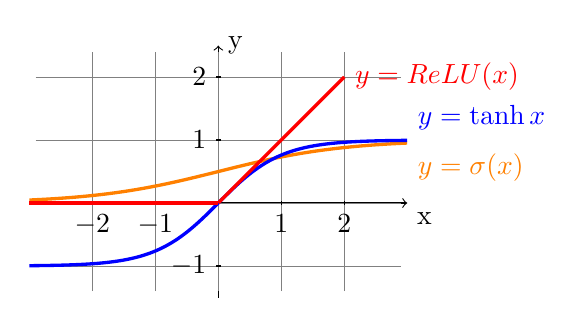
\begin{tikzpicture}[scale=0.8]
  % Draw axes
  \draw[->] (-3,0) -- (3,0) node[below right] {x};
  \draw[->] (0,-1.5) -- (0,2.5) node[right] {y};

  % Draw gridlines
  \draw[step=1cm,gray,very thin] (-2.9,-1.4) grid (2.9, 2.4);

  \foreach \x in {-2,-1,1,2}
    \draw (\x cm,1pt) -- (\x cm,-1pt) node[anchor=north] {$\x$};
  \foreach \y in {-1,  1, 2}
    \draw (1pt, \y cm) -- (-1pt, \y cm) node[anchor=east] {$\y$};

  % Draw sigmoid
  \draw[orange, very thick, domain=-3:3, samples=200] plot (\x, {1/(1+exp(-\x))})
    node[below right] {$y=\sigma(x)$};

  % Draw Tanh
  \draw[blue, very thick, domain=-3:3, samples=200] plot (\x, {(exp(\x)-exp(-\x))/(exp(\x)+exp(-\x))})
    node[above right] {$y=\tanh{x}$};

  % Draw ReLU
  \draw[red, very thick, domain=-3:0, samples=5] plot (\x, {0});
  \draw[red, very thick, domain=0:2, samples=5] plot (\x, {\x}) node[right]
    {$y=\F{ReLU}(x)$};

\end{tikzpicture}
